\documentclass[t]{beamer}
\usetheme{Copenhagen}
\setbeamertemplate{headline}{} % remove toc from headers
\beamertemplatenavigationsymbolsempty

\usepackage{amsmath, array, tikz, bm, pgfplots, tcolorbox, graphicx, venndiagram, color, colortbl, xfrac}
\pgfplotsset{compat = 1.16}
\usepgfplotslibrary{statistics}
\usetikzlibrary{calc}

\title{Linear Regression}
\author{}
\date{}

\AtBeginSection[]
{
  \begin{frame}
    \frametitle{Objectives}
    \tableofcontents[currentsection]
  \end{frame}
}

\begin{document}

\begin{frame} 
\maketitle
\end{frame}

\section{Determine and interpret the linear correlation coefficient}

\begin{frame}{Linear Correlation Coefficient}
In the previous section, we examined correlation types (positive, negative, or none) with the help of the means of the explanatory ($x$) and response variables ($y$).	\newline\\	\pause

In this section, we will examine the correlation type the way it is done in the real world: calculating the linear correlation coefficient ($r$).	
\end{frame}

\begin{frame}{Linear Correlation Coefficient}
\begin{tcolorbox}[colframe=green!20!black, colback = green!30!white,title=\textbf{Correlation Coefficient}]
The \textbf{correlation coefficient}, $r$, is a numerical value with $-1 \leq r \leq 1$ that measures the type of linear correlation of a bivariate dataset.
\end{tcolorbox}
\bigskip 

\begin{itemize}
	\item<2->{$r > 0$: positive linear correlation}
	\item<3->{$r = 0$: no linear correlation}
	\item<4->{$r < 0$: negative linear correlation}
\end{itemize}
\end{frame}

\begin{frame}{Linear Correlation Coefficient}
\[r = \frac{\sum (x-\overline{x})(y-\overline{y})}{\sqrt{\sum(x-\overline{x})^2 \cdot \sum(y-\overline{y})^2}}\]	\newline\\	
\onslide<2->{We will use technology to calculate $r$}	\newline\\
\onslide<3->{The closer $r$ is to 1 (or $-1$), the more the data points ``fall in line"}	\newline\\
\onslide<4->{The closer $r$ is to 0, the more the data points resemble a ``cloud"}
\end{frame}

\begin{frame}{Interpreting $r$}
\begin{center}
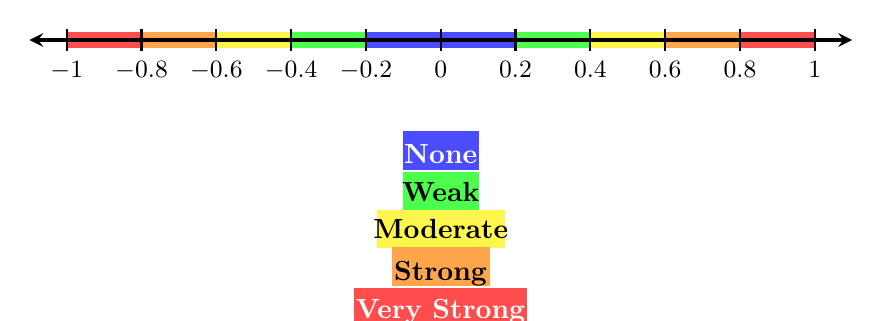
\begin{tikzpicture}[scale=0.95]
\draw [color=red!70, fill=red!70] (-5,-0.1) rectangle (5,0.1);
\draw [color=orange!70, fill=orange!70] (-4,-0.1) rectangle (4,0.1);
\draw [color=yellow!70, fill=yellow!70] (-3,-0.1) rectangle (3,0.1);
\draw [color=green!70, fill=green!70] (-2,-0.1) rectangle (2,0.1);
\draw [color=blue!70, fill=blue!70] (-1,-0.1) rectangle (1,0.1);
\draw [<->, >=stealth, very thick] (-5.5,0) -- (5.5,0);
\foreach \x in {-5,-4,...,5}
\draw [thick] (\x, 0.15) -- (\x,-0.15);
\node at (-5,-0.15) [below] {\small $-1$};
\node at (-4,-0.15) [below] {\small $-0.8$};
\node at (-3,-0.15) [below] {\small $-0.6$};
\node at (-2,-0.15) [below] {\small $-0.4$};
\node at (-1,-0.15) [below] {\small $-0.2$};
\node at (0,-0.15) [below] {\small $0$};
\node at (1,-0.15) [below] {\small $0.2$};
\node at (2,-0.15) [below] {\small $0.4$};
\node at (3,-0.15) [below] {\small $0.6$};
\node at (4,-0.15) [below] {\small $0.8$};
\node at (5,-0.15) [below] {\small $1$};
\raisebox{-0.5cm}{
\draw [color=blue!70, fill=blue!70] (-0.5,-1.2) rectangle (0.5,-0.7);
\node at (0,-1) {\color{white}\textbf{None}};
\draw [color=green!70, fill=green!70] (-0.5,-1.75) rectangle (0.5,-1.25);
\node at (0,-1.5) {\color{black}\textbf{Weak}};
\draw [color=yellow!70, fill=yellow!70] (-0.85,-2.25) rectangle (0.85,-1.75);
\node at (0,-2) {\color{black}\textbf{Moderate}};
\draw [color=orange!70, fill=orange!70] (-0.65,-2.75) rectangle (0.65,-2.25);
\node at (0,-2.6) {\color{black}\textbf{Strong}};
\draw [color=red!70, fill=red!70] (-1.15,-3.35) rectangle (1.15,-2.8);
\node at (0,-3.1) {\color{white}\textbf{Very Strong}}; }
\end{tikzpicture}
\end{center}
\bigskip
\onslide<2->{\emph{Note:} These interpretations are not universal.}
\end{frame}

\begin{frame}{Example 1}
Find and interpret the linear correlation coefficient, $r$, for each.	\newline\\
(a) \newline
\begin{minipage}{0.3\textwidth}
\scalebox{0.8}{
\begin{tabular}{c|c}
$x$ & $y$ \\ \hline
7.6 & 19.1 \\
9.2 & 22.9 \\
3.3 & 10.3 \\
1.1 & 6.6 \\
3.7 & 10.6 \\
3.9 & 11.3 \\
4.6 & 12.9 \\
2.3 & 8.6 \\
5.1 & 15.2 \\
5.3 & 15.1 \\
2.5 & 13 \\
3.4 & 11.2 \\
3.1 & 10.6 \\
1.7 & 6.8 \\
3.7 & 13.7 \\
\end{tabular} }
\end{minipage}
\begin{minipage}{0.55\textwidth}
\onslide<2->{$r \approx 0.9588$} \\[8pt]
\onslide<3->{Very strong positive linear correlation} \\[8pt]
\onslide<4->{
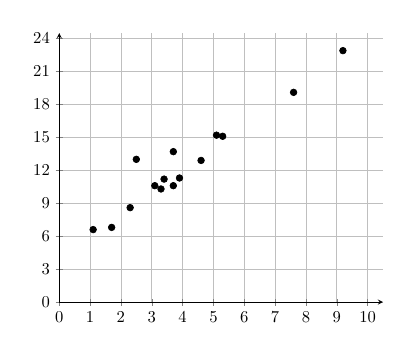
\begin{tikzpicture}[scale=0.6]
	\begin{axis}[
	axis lines = left, grid,
	xmin = 0, xmax = 10.5,
	ymin = 0, ymax = 24.5,
	xtick = {0,1,...,10},
	ytick = {0,3,...,24}
	]
\addplot [only marks] coordinates {
(7.6, 19.1)
(9.2, 22.9)
(3.3, 10.3)
(1.1, 6.6)
(3.7, 10.6)
(3.9, 11.3)
(4.6, 12.9)
(2.3, 8.6)
(5.1, 15.2)
(5.3, 15.1)
(2.5, 13)
(3.4, 11.2)
(3.1, 10.6)
(1.7, 6.8)
(3.7, 13.7)
};
\end{axis}
\end{tikzpicture}
}
\end{minipage}
\end{frame}

\begin{frame}{Example 1}
(b) \newline
\begin{minipage}{0.3\textwidth}
\scalebox{0.9}{
\begin{tabular}{c|c}
$x$ & $y$ \\ \hline
7.6 & 11.0 \\
9.2 & 3.6 \\
6.3 & 8.9 \\
1.1 & 14.9\\
6.7 & 8.1 \\
3.9 & 12.0 \\
4.6 & 9.4 \\
2.3 & 10.3 \\
5.1 & 11.4 \\
5.3 & 12.4 \\
2.5 & 9.0 \\
3.4 & 8.9 \\
3.1 & 14.2 \\
1.7 & 10.9 \\
3.7 & 13.3 \\
\end{tabular} }
\end{minipage}
\begin{minipage}{0.5\textwidth}
\onslide<2->{$r \approx -0.6273$} \\[8pt]
\onslide<3->{Strong negative linear correlation} \\[8pt]
\onslide<4->{
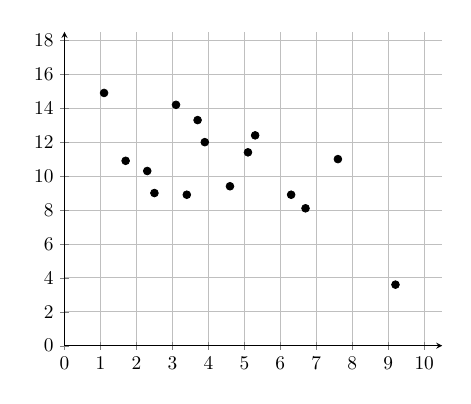
\begin{tikzpicture}[scale=0.7]
	\begin{axis}[
	axis lines = left, grid,
	xmin = 0, xmax = 10.5,
	ymin = 0, ymax = 18.5,
	xtick = {0,1,...,10},
	ytick = {0,2,...,18}
	]
\addplot [only marks] coordinates{
(7.6, 11.0)
(9.2, 3.6)
(6.3, 8.9)
(1.1, 14.9)
(6.7, 8.1)
(3.9, 12.0)
(4.6, 9.4)
(2.3, 10.3)
(5.1, 11.4)
(5.3, 12.4)
(2.5, 9.0)
(3.4, 8.9)
(3.1, 14.2)
(1.7, 10.9)
(3.7, 13.3)
};
\end{axis}
\end{tikzpicture}
}
\end{minipage}
\end{frame}

\begin{frame}{Example 1}
(c) \newline
\begin{minipage}{0.3\textwidth}
\scalebox{0.9}{
\begin{tabular}{c|c}
$x$ & $y$ \\ \hline
6.9 & 3.4 \\
7.7 & 4.5 \\
0.9 & 9.8 \\
3.4 & 1.5 \\
8.9 & 3.3 \\
5.7 & 8.9 \\
3.1 & 8.4 \\
2.2 & 8.1 \\
4.5 & 6.8 \\
4.1 & 0.5 \\
5.0 & 0.4 \\
7.8 & 8.4 \\
2.5 & 3.1 \\
6.1 & 9.0 \\
1.1 & 8.5 \\
\end{tabular} }
\end{minipage}
\begin{minipage}{0.5\textwidth}
\onslide<2->{$r \approx -0.2218$} \\[8pt]
\onslide<3->{Weak negative correlation} \\[8pt]
\onslide<4->{
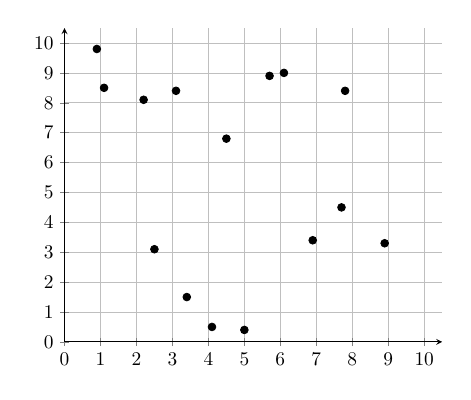
\begin{tikzpicture}[scale=0.7]
	\begin{axis}[
	axis lines = left, grid,
	xmin = 0, xmax = 10.5,
	ymin = 0, ymax = 10.5,
	xtick = {0,1,...,10},
	ytick = {0,1,...,10}
	]
\addplot [only marks] coordinates{
(6.9, 3.4)
(7.7, 4.5)
(0.9, 9.8)
(3.4, 1.5)
(8.9, 3.3)
(5.7, 8.9)
(3.1, 8.4)
(2.2, 8.1)
(4.5, 6.8)
(4.1, 0.5)
(5.0, 0.4)
(7.8, 8.4)
(2.5, 3.1)
(6.1, 9.0)
(1.1, 8.5)
};
\end{axis}
\end{tikzpicture}
}
\end{minipage}
\end{frame}

\section{Determine the linear regression equation}

\begin{frame}{Linear Regression Equation}
While determining the linear correlation coefficient is valuable, it is also helpful to be able to predict data values not contained in the data set. \newline\\	\pause

To do this, we can create the {\color{blue}\textbf{least squares regression equation}}, (also called the \emph{line of best fit}) which will \alert{\textbf{minimize}} the total squared distance each data point is from the line:	\pause

\[\hat{y} = mx + b\]
\end{frame}

\begin{frame}{Line of Best Fit}
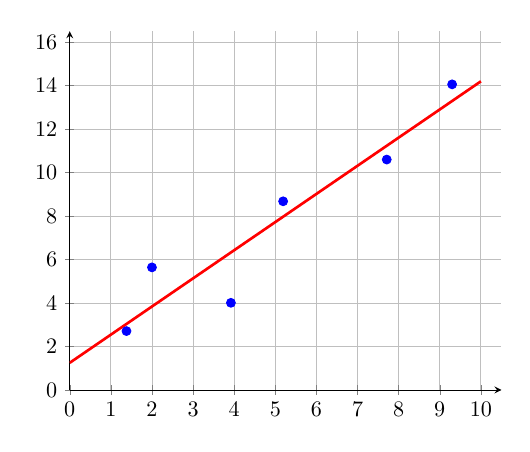
\begin{tikzpicture}[scale=0.8]
\begin{axis}[
	axis lines = left, grid,
	xmin = 0, xmax = 10.5, ymin = 0, ymax = 16.5,
	xtick = {0,1,...,10}, ytick = {0,2,...,16}
]
\addplot[color=blue, only marks] coordinates {
(9.3,14.06)
(5.19,8.68)
(2,5.64)
(7.71,10.6)
(1.38,2.71)
(3.92,4.01)
};
\addplot [color=red, domain=0:10, very thick] {1.295*x + 1.25};
\end{axis}
\end{tikzpicture}
\end{frame}

\begin{frame}{Least Squares Regression Equation}
\begin{minipage}{0.6\textwidth}
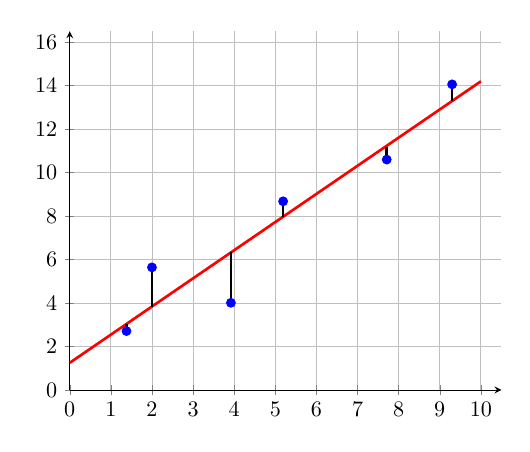
\begin{tikzpicture}[scale=0.8]
\begin{axis}[
	axis lines = left, grid,
	xmin = 0, xmax = 10.5, ymin = 0, ymax = 16.5,
	xtick = {0,1,...,10}, ytick = {0,2,...,16}
]
\addplot[color=blue, only marks] coordinates {
(9.3,14.06)
(5.19,8.68)
(2,5.64)
(7.71,10.6)
(1.38,2.71)
(3.92,4.01)
};
\addplot [color=red, domain=0:10, very thick] {1.295*x + 1.25};
\draw [very thick] (axis cs: 9.3,14.06) -- (axis cs: 9.3,13.3);
\draw [very thick] (axis cs: 7.71,10.6) -- (axis cs: 7.71,11.2);
\draw [very thick] (axis cs: 5.19,7.97) -- (axis cs: 5.19,8.68);
\draw [very thick] (axis cs: 3.92,4.01) -- (axis cs: 3.92,6.33);
\draw [very thick] (axis cs: 2,5.64) -- (axis cs: 2,3.84);
\draw [very thick] (axis cs: 1.38,2.71) -- (axis cs: 1.38,3.04);
\end{axis}
\end{tikzpicture}
\end{minipage}
\begin{minipage}{0.35\textwidth}
\onslide<2->{The black lines are {\color{blue}\textbf{residuals}}.} \\[8pt]
\onslide<3->{Like deviations from the mean, the sum of the residuals is 0.} \\[8pt]
\onslide<4->{So we need to square the deviations so the negatives don't cancel the positives.}
\end{minipage}
\end{frame}

\begin{frame}{Least Squares Regression Equation}
\begin{minipage}{0.6\textwidth}
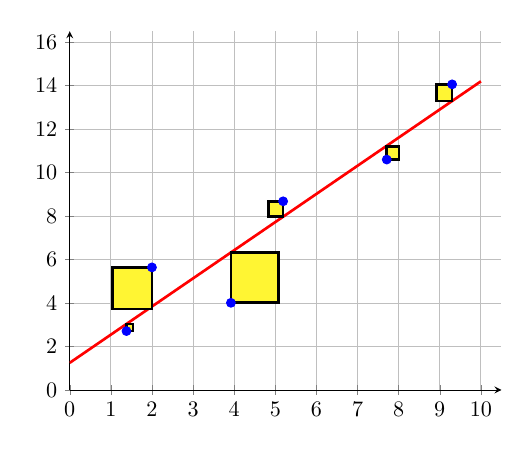
\begin{tikzpicture}[scale=0.8]
\begin{axis}[
	axis lines = left, grid,
	xmin = 0, xmax = 10.5, ymin = 0, ymax = 16.5,
	xtick = {0,1,...,10}, ytick = {0,2,...,16}
]
\addplot[color=blue, only marks] coordinates {
(9.3,14.06)
(5.19,8.68)
(2,5.64)
(7.71,10.6)
(1.38,2.71)
(3.92,4.01)
};
\addplot [color=red, domain=0:10, very thick] {1.295*x + 1.25};
\draw [very thick, fill=yellow!80] (axis cs: 9.3,14.06) rectangle +(axis cs: -0.38,-0.76);
\draw [very thick, fill=yellow!80] (axis cs: 7.71,10.6) rectangle +(axis cs: 0.3,0.6);
\draw [very thick, fill=yellow!80] (axis cs: 5.19,8.68) rectangle +(axis cs: -0.35,-0.71);
\draw [very thick, fill=yellow!80] (axis cs: 3.92,4.01) rectangle +(axis cs: 1.16,2.32);
\draw [very thick, fill=yellow!80] (axis cs: 2,5.64) rectangle +(axis cs: -0.96,-1.92);
\draw [very thick, fill=yellow!80] (axis cs: 1.38,2.71) rectangle +(axis cs: 0.16,0.33);
\end{axis}
\end{tikzpicture}
\end{minipage}
\begin{minipage}{0.35\textwidth}
\onslide<2->{The line of best fit minimizes the sum of the areas of the squares.} \\[8pt]
\end{minipage}
\end{frame}

\begin{frame}{Slope and $y$-intercept}
\textbf{We will be using technology to find the equation of the line of best fit.} \newline\\	\pause

Below are the formulas for calculating the slope, $m$, and $y$-intercept, $b$:	\pause
\[m = \frac{n(\sum xy) - (\sum x)(\sum y)}{n(\sum x^2) - (\sum x)^2}\]
\center{and}
\[b = \frac{(\sum y)(\sum x^2) - (\sum x)(\sum xy)}{n(\sum x^2) - (\sum x)^2}\]
\end{frame}

\begin{frame}{Example 2}
Find the least squares regression equation for the following dataset.	\newline\\
\begin{minipage}{0.3\textwidth}
\scalebox{0.8}{
\begin{tabular}{c|c}
$x$ & $y$ \\ \hline
7.6 & 19.1 \\
9.2 & 22.9 \\
3.3 & 10.3 \\
1.1 & 6.6 \\
3.7 & 10.6 \\
3.9 & 11.3 \\
4.6 & 12.9 \\
2.3 & 8.6 \\
5.1 & 15.2 \\
5.3 & 15.1 \\
2.5 & 13 \\
3.4 & 11.2 \\
3.1 & 10.6 \\
1.7 & 6.8 \\
3.7 & 13.7 \\
\end{tabular} }
\end{minipage}
\begin{minipage}{0.55\textwidth}
\onslide<2->{$\hat{y} = 1.95x + 4.65$} \\[10pt]
\onslide<3->{
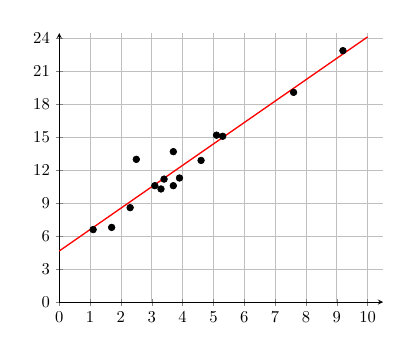
\begin{tikzpicture}[scale=0.6]
	\begin{axis}[
	axis lines = left, grid,
	xmin = 0, xmax = 10.5,
	ymin = 0, ymax = 24.5,
	xtick = {0,1,...,10},
	ytick = {0,3,...,24}
	]
\addplot [only marks] coordinates {
(7.6, 19.1)
(9.2, 22.9)
(3.3, 10.3)
(1.1, 6.6)
(3.7, 10.6)
(3.9, 11.3)
(4.6, 12.9)
(2.3, 8.6)
(5.1, 15.2)
(5.3, 15.1)
(2.5, 13)
(3.4, 11.2)
(3.1, 10.6)
(1.7, 6.8)
(3.7, 13.7)
};
\addplot [color=red, thick, domain=0:10] {1.95*x+4.65};
\end{axis}
\end{tikzpicture}
}
\end{minipage}
\end{frame}

\begin{frame}{Example 3}
Given the regression equation $\hat{y} = 1.95x + 4.65$, predict the values of the following response variables for each explanatory variable.	\newline\\
(a) \quad $x = 6$	\newline\\	\pause

Since 6 between the minimum and maximum values of $x$ in our dataset, finding its $y$-coordinate is called {\color{blue}\textbf{interpolation}}.	

\begin{align*}
\onslide<3->{\hat{y} &= 1.95x + 4.65} \\[6pt]
\onslide<4->{&= 1.95(6) + 4.65}.\\[6pt]
\onslide<5->{&= 16.35} 
\end{align*}

\onslide<6->{The predicted value when $x = 6$ is $y = 16.35$}
\end{frame}

\begin{frame}{Residuals}
Suppose we actually obtain a datapoint and realize that the actual value of $y$ when $x = 6$ is 16, not the predicted 16.35.	\newline\\	\pause

The residual, denoted $\epsilon$, would be 
\begin{align*}
\epsilon &= 16.35 - 16 \\[6pt]
\epsilon &= 0.35
\end{align*}
\pause

We could then add that observation to our dataset and use it to create a better linear regression equation.
\end{frame}

\begin{frame}{Example 3}
(b) \quad $x = 11$	\newline\\
\onslide<2->{Since 11 is outside of the $x$ values in our dataset, finding its $y$-coordinate is called {\color{blue}\textbf{extrapolation}}.}	

\begin{align*}
\onslide<3->{\hat{y} &= 1.95x + 4.65} \\[6pt]
\onslide<4->{&= 1.95(11) + 4.65} \\[6pt]
\onslide<5->{&= 26.1}
\end{align*}

\onslide<6->{The predicted value when $x = 11$ is $y = 26.1$.}
\end{frame}

\section{Determine and Interpret the Coefficient of Determination}


% Calculate r^2

\end{document}